\documentclass[frontgrid]{flacards}
\usepackage{color} 
\usepackage{graphicx}
\usepackage[notextcomp]{kpfonts} 
\usepackage{amsthm,amssymb,amsmath}
\usepackage{graphicx}
\usepackage{enumitem}
\usepackage{bm}
\usepackage{tabu}
\usepackage{mathtools}
\usepackage{tikz}
\usepackage{tikz-3dplot}
\usepackage{xcolor}
\usepackage{colortbl}
\usepackage{wasysym}

\begin{document}

\pagesetup{2}{3} 

%%%%% Domain, Range, Pairs of points on a graph

\card{Consider the following equation: \[f(x)=\sqrt{3x-5}\] Answer the following questions:\\ Domain:\\  Range:\\ List three pairs of points on the graph:}{functions}
\card{Consider the following equation: \[g(x)=\frac{2x+1}{x^2+5x+4}\] Answer the following questions:\\ Domain:\\  Range:\\ List three pairs of points on the graph:}{functions}
\card{Consider the following equation: \[h(x)=\sqrt{7-2x}\] Answer the following questions:\\ Domain:\\  Range:\\ List three pairs of points on the graph:}{functions}
\card{Consider the following equation: \[k(x)=\frac{x^2-4x+7}{x^2+16x+5}\] Answer the following questions:\\ Domain:\\  Range:\\ List three pairs of points on the graph:}{functions}

%%%%% Evaluating Functions

\card{Consider the following function: \[f(x)=8x-4x^2\] Evaluate the following questions:\\ Evaluate $f(4)$\\ Evaluate $f(a)$\\ Evaluate $f(4-a)$}{functions}
\card{Consider the following function: \[g(x)=2x^2-13x+28\] Evaluate the following questions:\\ Evaluate $g(8)$\\ Evaluate $f(h)$\\ Evaluate $f(h-8)$}{functions}
\card{Consider the following function: \[h(x)=7x^2-4x+5\] Evaluate the following questions:\\ Evaluate $h(9)$\\ Evaluate $h(b)$\\ Evaluate $f(b-9)$}{functions}
\card{Consider the following function: \[k(x)=3x^2-8x+17\] Evaluate the following questions:\\ Evaluate $k(3)$\\ Evaluate $k(c)$\\ Evaluate $k(c-3)$}{functions}

%%%%% Function
\card{\textbf{Answer the following questions:}\\ Draw a graph that represents a function. \\ Draw a graph that does not represent a function.\\ Create a table that represents a function.\\  Create a table that does not represent a function.}{functions} 
\card{\textbf{Answer the following questions:}\\ Draw a graph that represents a function. \\ Draw a graph that does not represent a function.\\ Write an equation that represents a function.\\ Write an equation that does not represent a function.}{functions}
\card{\textbf{Answer the following questions:}\\ Write an equation that represents a function.\\ Write an equation that does not represent a function.\\ Create a table that represents a function.\\  Create a table that does not represent a function.}{functions} 
\card{\textbf{Answer the following questions:}\\ Draw a graph that represents a function. \\ Draw a graph that does not represent a function.\\ Create a table that represents a function.\\  Create a table that does not represent a function.}{functions} 

%%%%% Linear Stuff 
\card{A new car salesperson is paid a monthly salary of \$800 plus a commission of 5\% of all the sales they make that month. Answer the following questions:\\ Write an equation that represents this situation.\\ What monthly sales amount would give the salesperson \$1,500?\\ How much will the salesperson make if they sell \$36,000 worth of cars?}{Linear}
\card{A jewelry salesperson is paid a monthly salary of \$1200 plus a commission of 1\% of all the sales they make that month. Answer the following questions:\\ Write an equation that represents this situation.\\ What monthly sales amount would give the salesperson \$3,000?\\ How much will the salesperson make if they sell \$12,000 worth of jewelry?}{Linear}
\card{A pair of jeans that costs, $P$ dollars, is placed on sale at a discount of 35\% off. If the sales tax is 8\%. Answer the following questions:\\ Write a function that represents the final sales price, $F$, as a function of $P$.\\ If the final sales cost was \$45, what was the original cost of the jeans?\\ How much would a pair of jeans cost that was originally \$100?}{Linear}
\card{A cardigan that costs, $P$ dollars, is placed on sale at a discount of 15\% off. If the sales tax is 12\%. Answer the following questions:\\ Write a function that represents the final sales price, $F$, as a function of $P$.\\ If the final sales cost was \$70, what was the original cost of the cardigan?\\ How much would a cardigan cost that was originally \$80?}{Linear}

%%%%% Graphs
\card{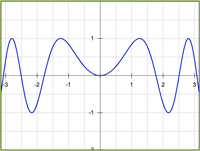
\includegraphics[scale=0.5]{graph1}\\ Describe the following features of the above graph:\\ Increasing, Decreasing, Constant:\\ Positive, Negative:\\ Domain, Range:\\ Evaluate: $f(0)$, $f(-2)$, $f(3)$}{Graphs}
\card{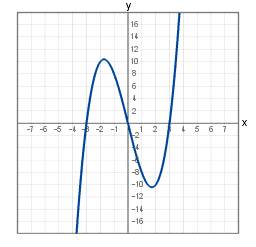
\includegraphics[scale=0.45]{graph2}\\ Describe the following features of the above graph:\\ Increasing, Decreasing, Constant:\\ Positive, Negative:\\ Domain, Range:\\ Evaluate: $f(-3)$, $f(2)$, $f(0)$}{Graphs}
\card{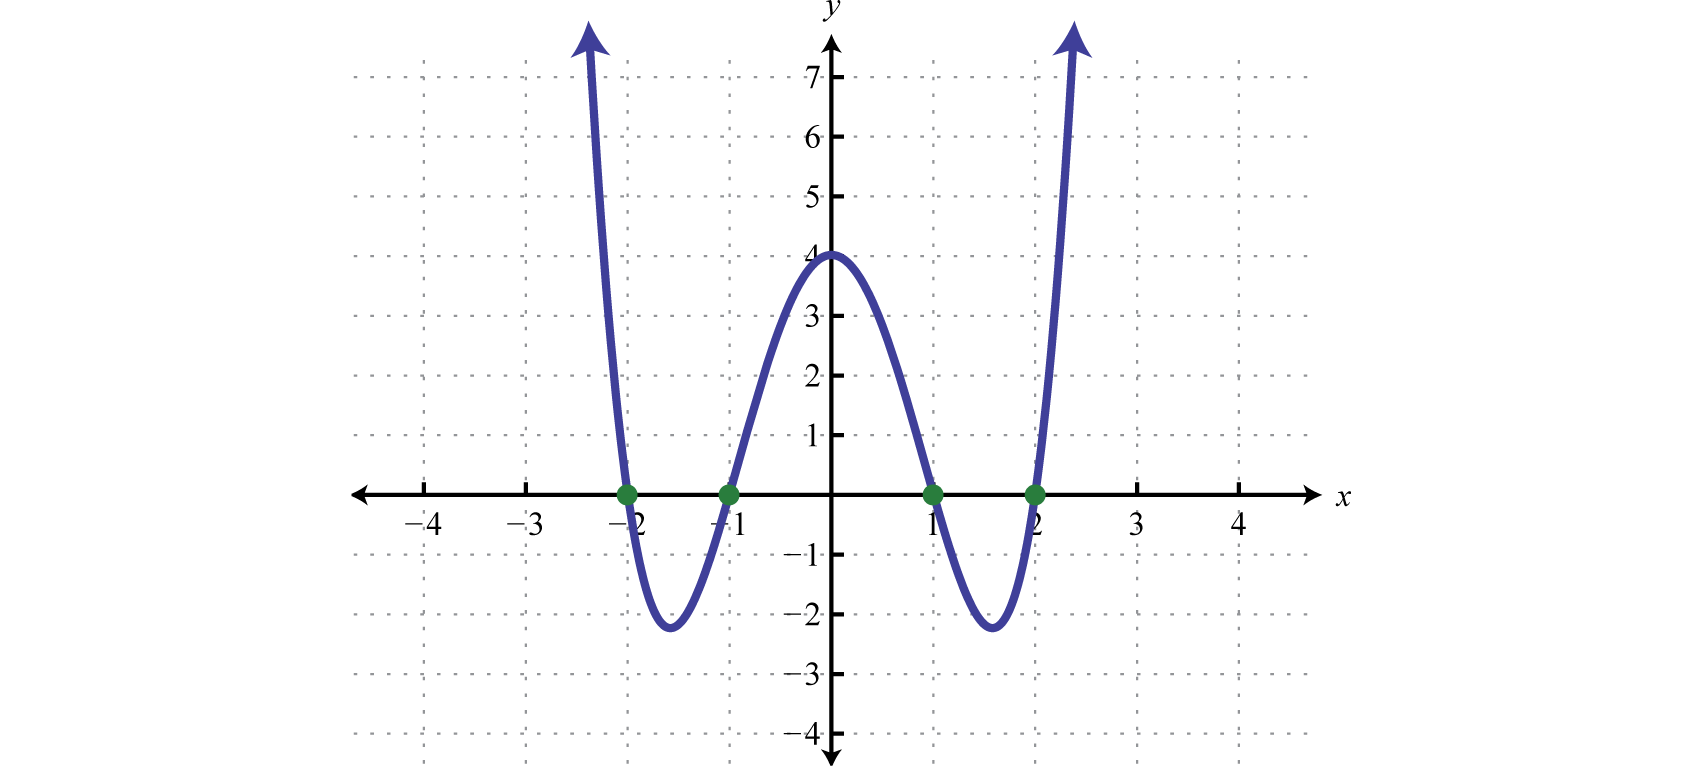
\includegraphics[scale=0.5]{graph3}\\ Describe the following features of the above graph:\\ Increasing, Decreasing, Constant:\\ Positive, Negative:\\ Domain, Range:\\ Evaluate: $f(0)$, $f(-1)$, $f(2)$}{Graphs}
\card{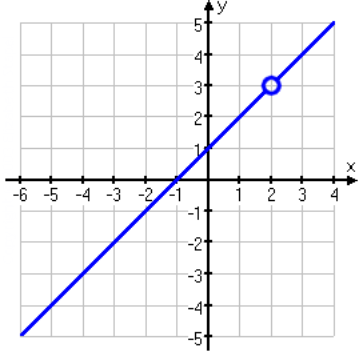
\includegraphics[scale=0.25]{graph4}\\ Describe the following features of the above graph:\\ Increasing, Decreasing, Constant:\\ Positive, Negative:\\ Domain, Range:\\ Evaluate: $f(0)$, $f(2)$, $f(-5)$}{Graphs}
\card{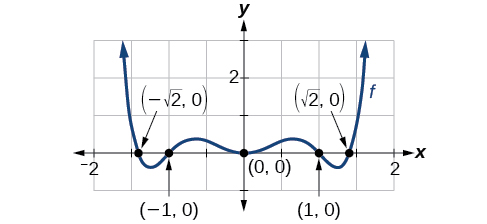
\includegraphics[scale=0.5]{graph5}\\ Describe the following features of the above graph:\\ Increasing, Decreasing, Constant:\\ Positive, Negative:\\ Domain, Range:\\ Determine the $x$-intercepts}{Graphs}
\card{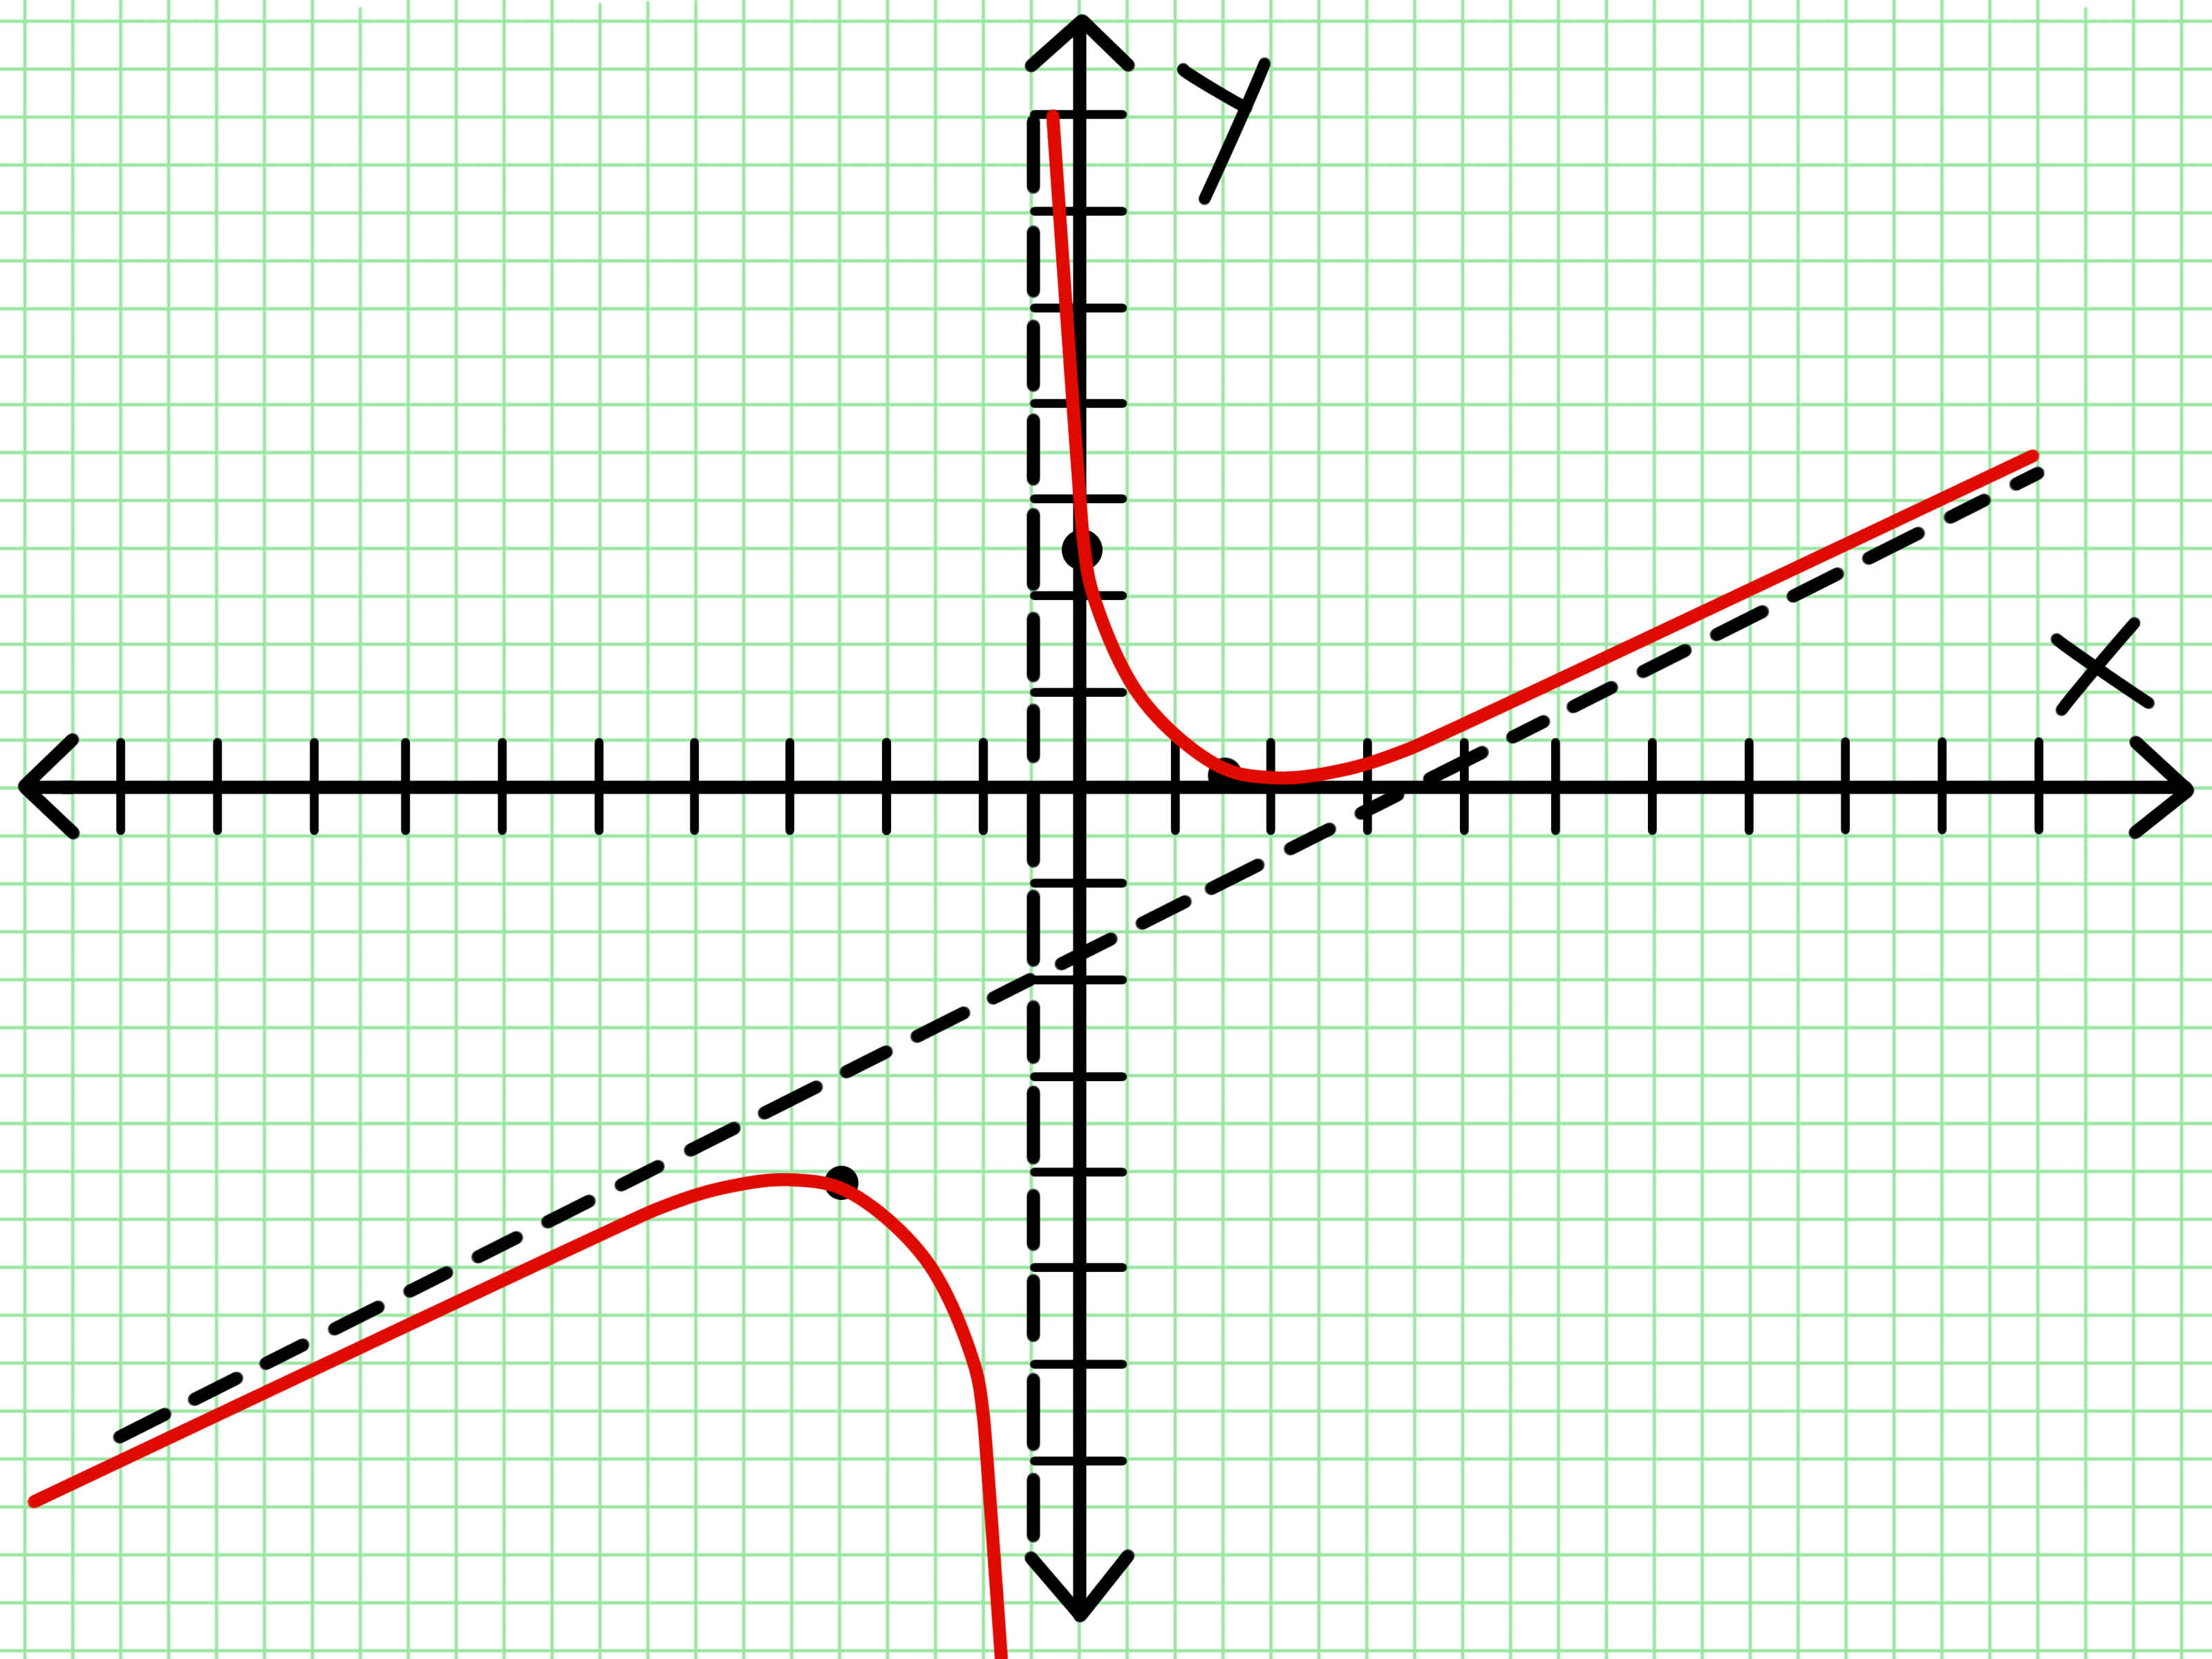
\includegraphics[scale=0.15]{graph6}\\ Describe the following features of the above graph:\\ Increasing, Decreasing, Constant:\\ Positive, Negative:\\ Domain, Range:\\ Determine the $x$-intercepts}{Graphs}
\card{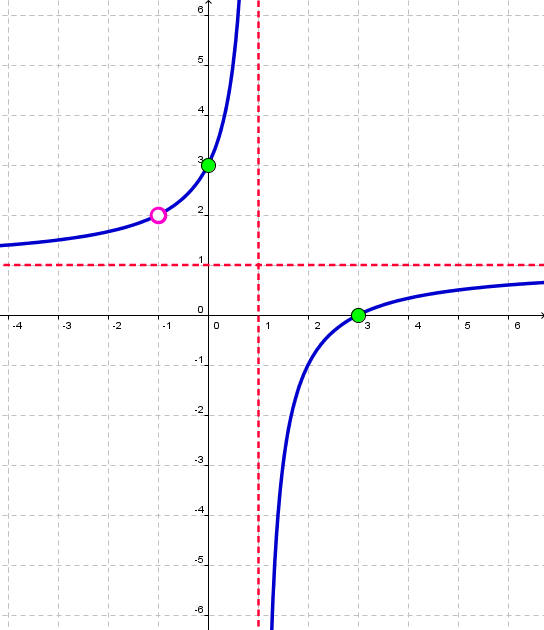
\includegraphics[scale=0.20]{graph7}\\ Describe the following features of the above graph:\\ Increasing, Decreasing, Constant:\\ Positive, Negative:\\ Domain, Range:\\ Evaluate: $f(-1)$, $f(2)$, $f(0)$}{Graphs}
\card{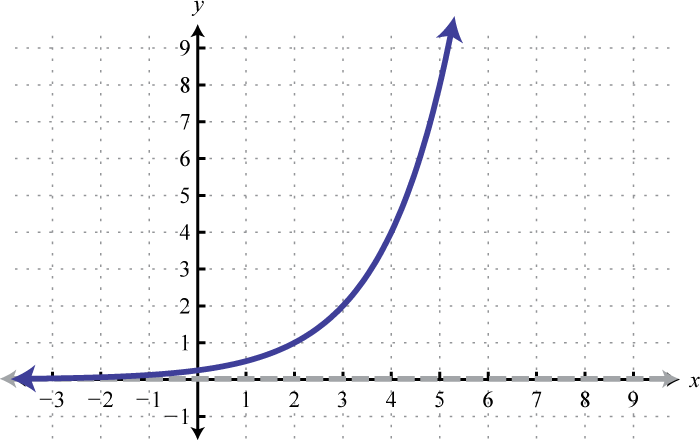
\includegraphics[scale=0.75]{graph8}\\ Describe the following features of the above graph:\\ Increasing, Decreasing, Constant:\\ Positive, Negative:\\ Domain, Range:}{Graphs}


%%%%% Graphs with your own calculator
\card{A manufacturer for socks estimates that the profit for selling $x$ pairs of socks is given by the function $P(x)=-\frac{1}{50}x^2+258x-38,250$. Answer the following questions:\\ Find the $x$-intercepts.\\ What do the $x$-intercepts mean in context of the problem.\\ Where is the graph increasing? Decreasing?\\ What is an appropriate domain? Range?\\ How many pairs of socks do they need to sell to maximize profit?\\ How much will they make if they maximize profit?}{Graphs}
\card{A manufacturer for stuffed animals estimates that the profit for selling $x$ animals is given by the function $P(x)=-\frac{1}{25}x^2+156x-27,540$. Answer the following questions:\\ Find the $x$-intercepts.\\ What do the $x$-intercepts mean in context of the problem.\\ Where is the graph increasing? Decreasing?\\ What is an appropriate domain? Range?\\ How many stuffed animals do they need to sell to maximize profit?\\ How much will they make if they maximize profit?}{Graphs}
\card{A manufacturer for bikes estimates that the profit for selling $x$ bikes is given by the function $P(x)=-\frac{1}{75}x^2+328x-54,746$. Answer the following questions:\\ Find the $x$-intercepts.\\ What do the $x$-intercepts mean in context of the problem.\\ Where is the graph increasing? Decreasing?\\ What is an appropriate domain? Range?\\ How many bikes do they need to sell to maximize profit?\\ How much will they make if they maximize profit?}{Graphs}
\card{A manufacturer for cupcakes estimates that the profit for selling $x$ cupcakes is given by the function $P(x)=-\frac{1}{15}x^2+114-4,000$. Answer the following questions:\\ Find the $x$-intercepts.\\ What do the $x$-intercepts mean in context of the problem.\\ Where is the graph increasing? Decreasing?\\ What is an appropriate domain? Range?\\ How many pairs of cupcakes do they need to sell to maximize profit?\\ How much will they make if they maximize profit?}{Graphs}

%%%%% Lines!!
\card{Write an equation for the line that has a slope of $\frac{1}{2}$ and passes through the point $(2,-2)$}{Lines}
\card{Write an equation for the line that has a slope of $\frac{3}{4}$ and passes through the point $(-7,5)$}{Lines}
\card{Write an equation for the line that has a slope of $5$ and passes through the point $(4,8)$}{Lines}
\card{Write an equation for the line that has a slope of $10$ and passes through the point $(5,7)$}{Lines}
\card{Write an equation for the line that passes through the points $(2,-2)$ and $(3,4)$}{Lines}
\card{Write an equation for the line that passes through the points $(8,5)$ and $(4,6)$}{Lines}
\card{Write an equation for the line that passes through the points $(6,-8)$ and $(5,7)$}{Lines}
\card{Write an equation for the line that passes through the points $(-4,2)$ and $(-4,9)$}{Lines}
\card{Write an equation for the line that passes through the point $(2,-2)$ and has a slope of 0}{Lines}
\card{Write an equation for the line that passes through the point $(2,5)$ and has a slope of 0}{Lines}
\card{Write an equation for the line that passes through the points $(2,-2)$ and undefined slope}{Lines}
\card{Write an equation for the line that passes through the points $(7,9)$ and has an undefined slope}{Lines}
\card{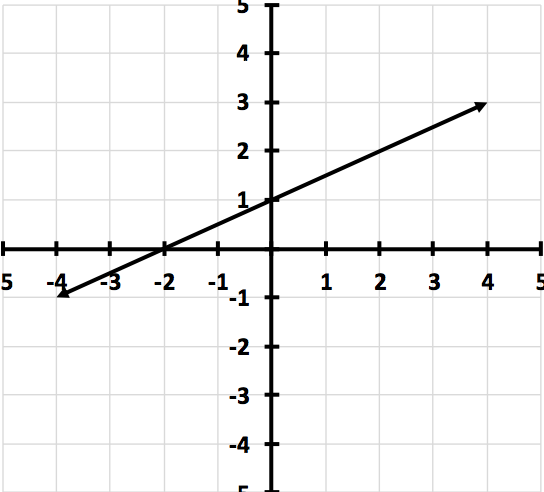
\includegraphics[scale=0.5]{line}\\ Determine an equation for the linear function below\\ What is the $x$-intercept?\\ What is the $y$-intercept? }{Lines}
\card{A couple invests \$4,000 into an apiary. On average each pint of honey the apiary produces costs \$2.76 to produces and sells for \$10.20 per pint.\\ Answer the following questions:\\ Create a cost function.\\ Create a revenue function.\\ How many pints of honey does the couple need to sell in order to break even?}{Lines}
\card{A couple invests \$8,000 into an rollerskating rink. On average each person that comes into the rink costs the rink \$30 but will pay \$45.\\ Answer the following questions:\\ Create a cost function.\\ Create a revenue function.\\ How many pints of honey does the couple need to sell in order to break even?}{Lines}
\card{A network is tracking the viewership of a new television show. After 5 weeks on the air, the number of viewers was 8,000,000. After another 5 weeks, the number of viewers had dropped to 6,000,000. Assume that the viewership has been decreasing linearly.\\ Write a function to model this situation.\\ Explain what the slope means in practical terms.}{Lines}
\card{A concert venue holds a maximum of 1000 people. With ticket prices at \$50, the average attendance is 600 people. For every \$5 the ticket price is lowered, approximately 25 more people attend. Write an equation to represent this situation.}{Lines}

%%%%% Piecewise
\card{Use the following piecewise equation to answer questions: \[ f(x) = \begin{cases} 
 2x-1 & \text{if } x <-2\\
 x+3 & \text{if } x \geq -2	
 \end{cases} \] Evaluate:\\ $g(0)$, $g(-3)$, $g(5)$\\ What is the $y$-intercept?\\ What is the $x$-intercept?\\ Graph the equation.\\ Domain? Range? }{Piecewise}
\card{Use the following piecewise equation to answer questions: \[ f(x) = \begin{cases} 
 x+2  & \text{if } x >1\\
 -3 & \text{if } x \leq 1	
 \end{cases} \] Evaluate:\\ $g(0)$, $g(-3)$, $g(5)$\\ What is the $y$-intercept?\\ What is the $x$-intercept?\\ Graph the equation.\\ Domain? Range? }{Piecewise}
\card{Use the following piecewise equation to answer questions: \[ f(x) = \begin{cases} 
 2x-3  & \text{if } x \leq 3\\
-\frac{1}{2}x+5 & \text{if } x > 3	
 \end{cases} \] Evaluate:\\ $g(0)$, $g(-3)$, $g(5)$\\ What is the $y$-intercept?\\ What is the $x$-intercept?\\ Graph the equation.\\ Domain? Range? }{Piecewise} 
\card{Use the following piecewise equation to answer questions: \[ f(x) = \begin{cases} 
 \frac{1}{3}x-1  & \text{if } x \neq -1\\
 5 & \text{if } x = -1	
 \end{cases} \] Evaluate:\\ $g(0)$, $g(-3)$, $g(5)$\\ What is the $y$-intercept?\\ What is the $x$-intercept?\\ Graph the equation.\\ Domain? Range? }{Piecewise}
\card{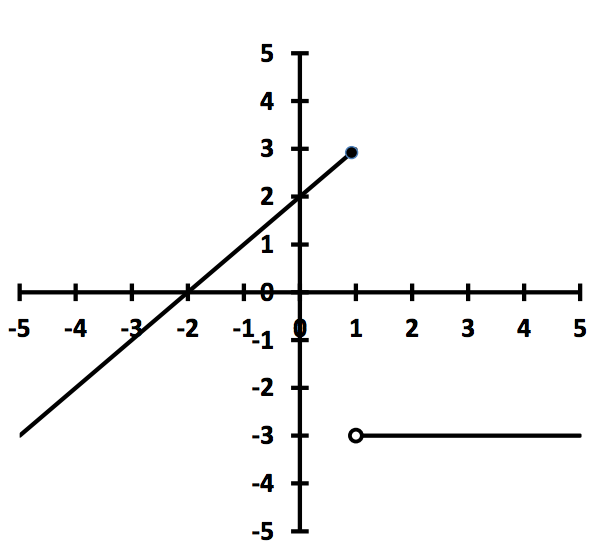
\includegraphics[scale=0.5]{Piecewise1}\\ Answer the following questions: What is the domain? Range?\\ Find a rule for the piecewise function.}{Piecewise}
\card{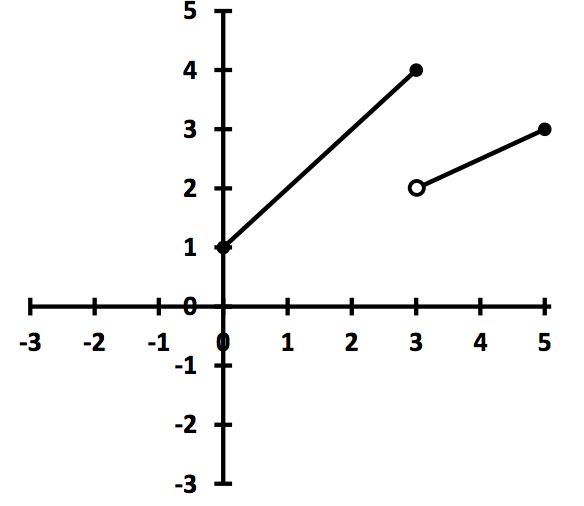
\includegraphics[scale=0.5]{Piecewise2}\\ Answer the following questions: What is the domain? Range?\\ Find a rule for the piecewise function.}{Piecewise} 
\card{Nell has a sales clerk job that pays \$15 per hour for regular work hours (less than or equal to 40 hours per week). She gets double time (or \$30 per hour) for any hours over 40 that she works in a week. Write a function that describes this function. What is the appropriate domain?}{Piecewise}
\card{Janet has a sales clerk job that pays \$20 per hour for regular work hours (less than or equal to 40 hours per week). She gets double time (or \$40 per hour) for any hours over 40 that she works in a week. Write a function that describes this function. What is the appropriate domain?}{Piecewise}
\card{An online novelty shop sells cheap fidget spinners in bulk. They charge \$2.25 each for the first 50 spinners, and \$1.75 each for any additional spinners. Write a function that describes this function. What is the appropriate domain? How many spinners could you buy for \$250? How much would it cost to buy 75 spinners?}{Piecewise}

%%%%% Transformations
\card{If $(3,-4)$ is a point on the graph of $y=f(x)$, what is the corresponding point of the graph\\ $y=-\frac{1}{3}f(x+5)-3$?\\ $y=4(\frac{1}{2}x)+2$?\\ $y=-f(x)$?}{Transformations} 
\card{If $(-2,7)$ is a point on the graph of $y=f(x)$, what is the corresponding point of the graph\\ $y=-\frac{1}{5}f(x-3)+7$?\\ $y=-2(3x)+2$?\\ $y=-f(x-4)$?}{Transformations} 
\card{Suppose $y=g(x)$ has a domain of $[-2,15)$ and a range of $[3, 10)$. Evaluate the domain and range of:\\ $y=-g(x)$\\ $y=g(-x)$\\ $y=g(x+4)-2$\\ $y=g(x-3)+5$}{Transformations}
\card{Suppose $y=g(x)$ has a domain of $[-5,13)$ and a range of $[-2, 12)$. Evaluate the domain and range of:\\ $y=-g(x)$\\ $y=g(-x)$\\ $y=g(x+2)-8$\\ $y=g(x-4)+1$}{Transformations}
\card{Write the base function and the transformations in order for the following functions:\\ $y=3(x-4)^2+1$\\ $y=\frac{1}{4}(\frac{1}{3}x)^3-1$\\ $y=-2\sqrt{x+5}+4$\\ $y=\frac{1}{2}\sqrt{2x}-5$  }{Transformations} 
\card{Write the base function and the transformations in order for the following functions:\\ $y=4(x-7)^2+8$\\ $y=\frac{2}{5}(2x)^3-1$\\ $y=-2\sqrt{x+5}+4$\\ $y=\frac{1}{2}\sqrt{\frac{2}{3}x}-5$}{Transformations} 
\card{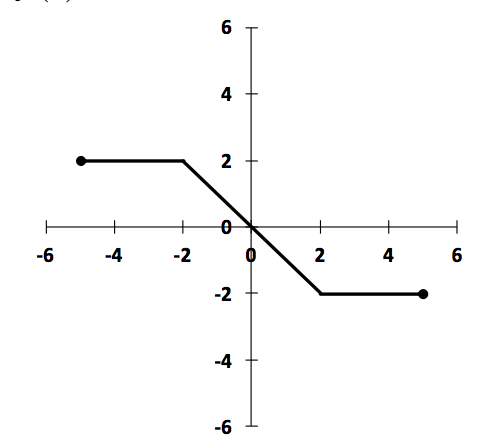
\includegraphics[scale=0.5]{Transformations1}\\ Graph the following transformations:\\ $y=-\frac{1}{3}f(x+5)-3$?\\ $y=4(\frac{1}{2}x)+2$?\\ $y=-f(x)$}{Transformations}
\card{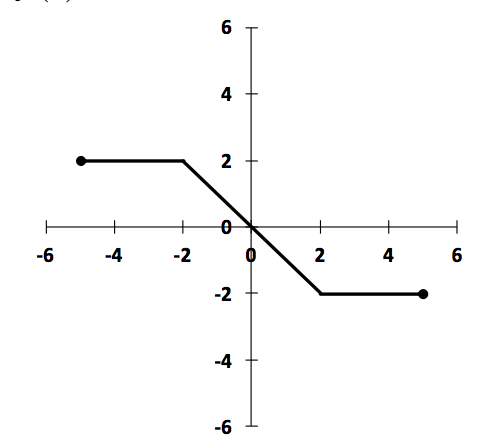
\includegraphics[scale=0.5]{Transformations1}\\ Graph the following transformations:\\ $y=-\frac{1}{5}f(x-3)+7$?\\ $y=-2(3x)+2$?\\ $y=-f(x-4)$}{Transformations}
\card{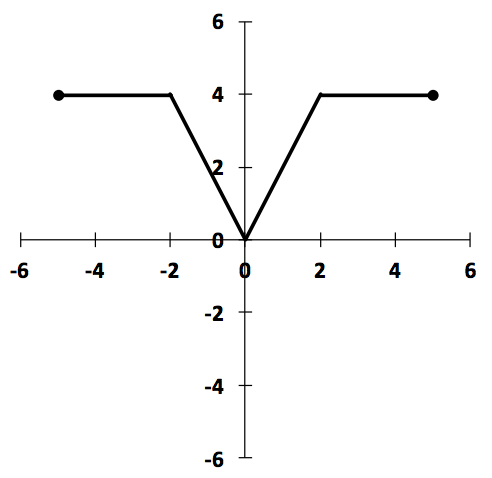
\includegraphics[scale=0.5]{Transformations2}\\ Graph the following transformations:\\ $y=-\frac{1}{5}f(x-3)+7$?\\ $y=-2(3x)+2$?\\ $y=-f(x-4)$}{Transformations} 
\card{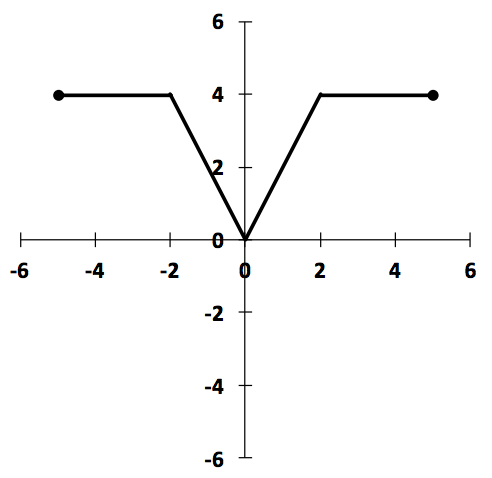
\includegraphics[scale=0.5]{Transformations2}\\ Graph the following transformations:\\ $y=-\frac{1}{3}f(x+5)-3$?\\ $y=4(\frac{1}{2}x)+2$?\\ $y=-f(x)$?}{Transformations} 
 
 
 
 
 
 
 
 
 
 
\end{document}
















